\documentclass[11pt,letterpaper]{article}
\usepackage[margin=0.75in]{geometry}
\usepackage{graphicx,amsmath,amssymb,booktabs,float,array,tabularx,placeins}
\usepackage[unicode,hidelinks]{hyperref}
\usepackage[T1]{fontenc}
\usepackage{lmodern}
\setlength{\parindent}{0pt}
\setlength{\parskip}{6pt}
\setlength{\emergencystretch}{3em}
\renewcommand{\topfraction}{0.92}
\renewcommand{\bottomfraction}{0.85}
\renewcommand{\textfraction}{0.08}
\renewcommand{\floatpagefraction}{0.8}
\hypersetup{pdftitle={Allogeneic screen performance and functional evidence for six autoimmune-screen β-cell candidates},pdfauthor={UCP Technology LLC}}
\begin{document}
{\LARGE\bfseries Allogeneic screen performance and functional evidence for six autoimmune-screen \(\beta\)-cell candidates\par}
\vspace{8pt}UCP Technology LLC | 25 October 2026\par
\section*{Abstract}
Immune protection and glucose-responsive secretion are distinct requirements for beta-cell replacement. We evaluated autoimmune-screen nominees in a published allogeneic screen and assessed functional evidence. Six of eleven mouse targets had mapped human counterparts among 11,689 gene scores. Their normalized Mann--Whitney statistic was theta = 0.421; a one-sided competitive random-set test did not detect positive enrichment (p = 0.744). A uniform, alias-aware search covered all eleven targets with citation checking. RNLS-edited human stem-cell-derived beta-like cultures showed improved CD45-negative cell survival after 72 hours with IL2-stimulated, HLA-mismatched PBMCs, a short-term benefit that does not establish durable graft protection or retained secretion. No adequate post-immune basal/stimulated secretion comparison was located in the assessed sources. Baseline findings included favorable responses and assays with unresponsive controls, without supplying post-immune comparisons. Autoimmune-screen nomination alone should not be treated as evidence of established allogeneic protection. The evidence map identifies candidate-specific uncertainties and measurements needed to connect protection with retained useful function.\par
\section*{Introduction}
A beta-cell edit can support persistence during immune attack without preserving useful insulin secretion. Baseline glucose responsiveness and retained function after challenge are also different observations. Candidate assessment requires evidence for protection, functional capacity, and their coexistence in the same experimental setting.\par
Cai et al. selected eleven surviving-guide targets in a mouse autoimmune CRISPR screen and independently validated RNLS, but reported no RNLS protection in their mouse allograft model [1]. Sintov et al. screened human stem-cell-derived islets exposed to unmatched peripheral blood mononuclear cells (PBMCs) [2]. RNLS/HIVEP2 spheroids lacked durable protection in allogeneic and xenogeneic graft settings [3]. Bode et al. found improved CD45-negative cell survival in RNLS-edited human beta-like cultures after 72 hours with IL2-stimulated, HLA-mismatched PBMCs [13], without establishing durable graft protection or retained secretion. RNLS metabolic studies also supplied baseline functional observations [4]. These context-dependent findings motivate cross-model comparison and experiment-specific functional assessment.\par
We ask whether eligible candidates rank unusually highly in the allogeneic screen, whether individuals meet its reported discovery threshold, and whether located experiments demonstrate protection with retained glucose responsiveness. This is a nominated-set analysis, not a comparison of complete genome-wide effect vectors. Species, cell product, maturation, graft conditions and immune effectors change together (Table 1), so rejection type is not isolated.\par
\begin{table}[!htbp]\centering\small
\renewcommand{\arraystretch}{1.15}
\begin{tabularx}{\linewidth}{@{}>{\raggedright\arraybackslash}X>{\raggedright\arraybackslash}X>{\raggedright\arraybackslash}X@{}}
\toprule
Dimension & Autoimmune discovery [1] & Allogeneic evaluation [2]\\\midrule
Cell product & Mouse NIT-1 insulinoma cells & Human stem-cell-derived mixed islet populations\\
Immune setting & NOD.scid recipients; diabetic NOD splenocyte transfer & MHC-null NSG recipients; unmatched human PBMCs\\
Graft and sampling & Subcutaneous NIT-1 grafts; retrieval at 8 weeks after immune transfer & Kidney capsule; retrieval at 10 weeks after PBMC injection\\
Screen output used here & Eleven selected surviving-guide target labels & 11,689 published gene scores from a KO-by-PBMC interaction model\\
Role in this study & Independent nomination and mapping denominator & Conditional rank comparison and original genome-wide adjusted q values\\
\bottomrule\end{tabularx}
\par\vspace{5pt}Table 1. The comparison supported by the available experiments. These are distinct cell and immune models, not a controlled contrast of rejection type. Separate validation experiments within each paper are evaluated individually in the functional evidence map.
\end{table}
\section*{Methods}
\subsection*{Eligibility and published measurements}
The primary plan fixed Cai Figure 1's eleven labels before candidate-score inspection: Hivep2, Rnls, Gcn1l1, Med11, Zbed3, Gm3604, Lgsn, Plin4, Tgm6, Grm2 and Olfr909. Frozen MGI/Alliance mapping resolved ten human counterparts, including Gcn1l1 to GCN1 and mapping-sensitive Gm3604 to ZNF28 [5]. No human counterpart was committed for Olfr909. Eligibility required a reported allogeneic score; missing scores were not imputed. All eleven targets remain in the functional assessment (Figure 1).\par
Sintov's Data S1 worksheet 'Fig3 - in vivo CRISPR screen' contains 11,689 unique, nonmissing gene scores. The source uses a negative-binomial KO-by-PBMC interaction model with mouse and guide random intercepts, non-targeting references and expression filtering [2]. We use the signed 'Fold change' field for direction and ordering because its exact export transformation is unconfirmed. The explicitly labeled -log10(FDR adj) field gives q = 10 to the power of its negative value. These are the source's genome-wide discovery q values.\par
\subsection*{Primary nominated-set statistic and uncertainty}
For reported universe U, candidates C, background B = U minus C, and score s, the normalized Mann--Whitney U statistic [7] is\par
\[\theta=\frac{\sum_{g\in C}\sum_{h\in B}[\mathbf{1}\{s_g>s_h\}+\frac{1}{2}\mathbf{1}\{s_g=s_h\}]}{|C|\,|B|}\]
Theta is the fraction of candidate-background comparisons favoring the candidate, counting ties by half. The directional hypothesis is theta > 0.5. The primary competitive reference samples one million size-six sets uniformly without replacement from U; the upper-tail p value uses the plus-one correction, with alpha = 0.05. The reference exchanges gene labels, not animals. Individual discovery support separately requires positive score and source q <= 0.05. Implementation details and full precision are supplied in the protocol and statistical supplement.\par
Inference is conditional on published point estimates; uncertainty in experimental effects, their ordering and biological reproducibility is not propagated. Monte Carlo error measures simulation error only. Nondetection does not establish equivalence or absence of benefit [8]. No nominal p values were reconstructed from adjusted q values for a new targeted test.\par
\subsection*{Calibration and assumption-specific secondary analyses}
Sensitivity analyses examine mapping, candidate omission and mouse-library eligibility. Secondary calibration summarizes the six-gene null distribution and the exact probability of drawing no genome-wide supported positive genes. Null-reference ranges are not biological confidence intervals.\par
Specified diffuse and sparse rank alternatives describe the design's detection frequency under explicit hypothetical distributions. They do not estimate biological power. The frozen secondary plan and statistical supplement retain all distribution parameters, seeds, sampling rules and Monte Carlo errors.\par
The secondary matched reference uses exact guide-count and control/pretransplant abundance-quintile strata among 11,474 genes with scores and covariates. Sampling preserves candidate counts within strata, and the statistic averages within-stratum superiority weighted by candidate count. This conditional estimand differs from the unrestricted primary. Control-graft abundance is measured after transplantation and can reflect biological selection, not merely technical coverage. Matching does not establish exchangeability or model intergene correlation; correlation-aware methods require experimental inputs beyond this score vector [9].\par
Descriptive count contrasts average log2(CPM + 1) within gene and animal before comparing groups, retaining all twelve mice [6]. Subtracting the shared non-targeting-guide contrast can change signs but not ordering. We compare published and descriptive ranks on the same 11,474 genes. Detailed annotation, sample-depth and omission diagnostics remain supplementary; this is not reconstruction of the source mixed model.\par
\subsection*{Bounded functional evidence assessment}
On 25 October 2026, we searched Europe PMC for each original target using the same title/abstract blocks for beta-cell context and secretion, function, glucose or immune protection. The target block combined original labels, current symbols, full names and human/mouse aliases from retained NCBI Gene records. First publication was bounded through that date, without a lower date limit. Exact strings, alias decisions, retrieval limits and screening dispositions are retained in the search protocol and logs. We also checked one generation of backward and forward citations around four biological anchor papers, reconciled indexed references with primary bibliographies, and followed relevant or ambiguous leads. Titles and available abstracts were screened; accessible primary text, figures and supplements supported extraction. Full-text source assessments were kept separate from extracted comparisons. These are bounded searches, not a claim of exhaustive systematic-review coverage; reporting follows applicable search-transparency principles [11,12].\par
Extraction separates observed glucose responsiveness, comparison with the relevant reference, and timing relative to immune challenge. It also records absolute versus ratio output, control responsiveness and protection. Favorable baseline observations are retained without promoting them to post-challenge claims. 'Not measured' denotes an absent endpoint in a located experiment; 'not located' denotes the search boundary. Gene--model--study rows preserve heterogeneous assays (Figure 4). Multiple gene rows from one pooled screen are not independent experiments.\par
Functional retention must name its reference: prechallenge output, a time-matched unchallenged edit, challenged unedited cells, or a justified useful-output threshold. Relative benefit over damaged controls need not imply adequate graft output. Total secretion, viable beta-cell mass and secretion per surviving cell are separate outcomes. Formal equivalence or noninferiority requires an appropriate margin and uncertainty analysis [10]; that requirement does not negate an observed baseline glucose response.\par
\section*{Results}
\subsection*{Eligibility and the primary comparison}
Six of eleven targets (54.5\%) were quantitatively eligible: HIVEP2, RNLS, GCN1, MED11, ZBED3 and ZNF28. LGSN, PLIN4, TGM6 and GRM2 were mapped but unscored; Olfr909 lacked a committed human mapping. These are coverage exclusions, not adverse effect estimates (Figure 1).\par
\begin{figure}[!htbp]\centering
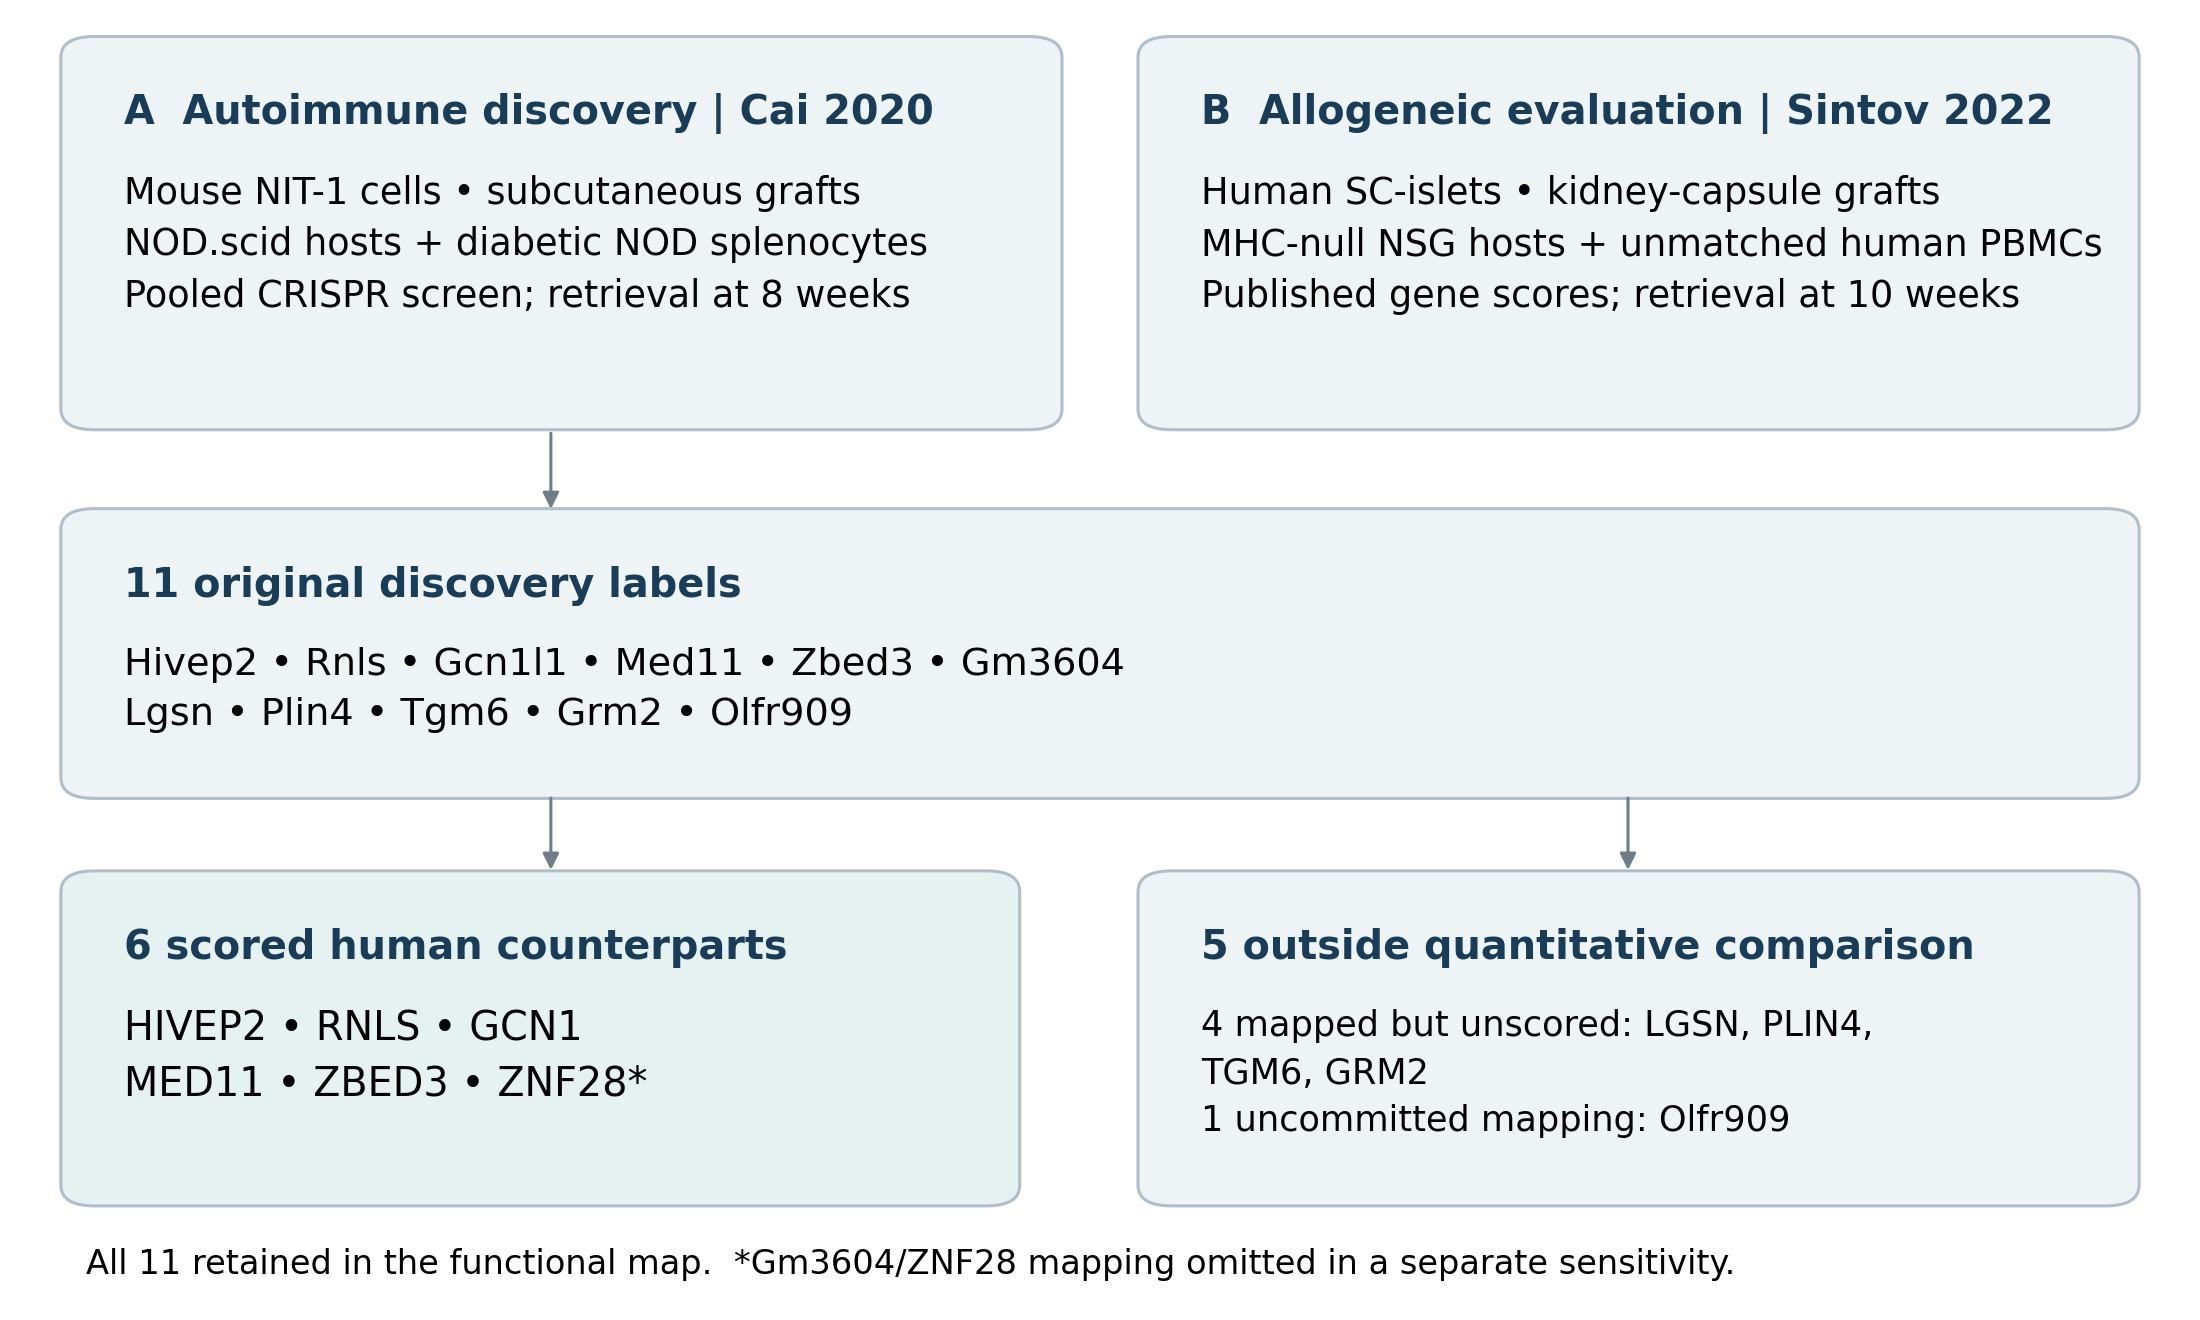
\includegraphics[width=\linewidth]{figures/eligibility.png}
\par\small Figure 1. Model comparison and eligibility. Eleven autoimmune discovery labels yield ten committed human mappings and six reported allogeneic scores. Mapping-sensitive Gm3604/ZNF28 remains in the primary set and is separately omitted in sensitivity analysis. All eleven original targets remain in functional assessment. The comparison does not isolate immune-challenge type.
\end{figure}
Primary theta was 0.421: candidate-background score comparisons favored the candidate in 42.1\% of pairs. The shift opposed the hypothesized direction, and the competitive test did not detect positive enrichment (one-sided p = 0.744; Figure 2). This does not establish depletion.\par
\begin{table}[!htbp]\centering\small
\renewcommand{\arraystretch}{1.15}
\begin{tabular}{lrrr}
\toprule
Gene & Signed score & Descending rank & Adjusted q\\\midrule
HIVEP2 & 0.188 & 2,279 & 0.830\\
RNLS & -0.142 & 7,704 & 0.872\\
GCN1 & 0.212 & 2,027 & 0.791\\
MED11 & -0.226 & 8,929 & 0.787\\
ZBED3 & -0.276 & 9,475 & 0.693\\
ZNF28 & -0.355 & 10,196 & 0.584\\
\bottomrule\end{tabular}
\par\vspace{5pt}Table 2. All six eligible candidates. Rank 1 is the largest signed score among 11,689 genes. These are descending signed-score ranks, not demonstrated protection ranks. Source genome-wide q values are retained; full precision is available in results/candidate\_scores.tsv.
\end{table}
GCN1 and HIVEP2 had positive scores; none met positive score plus genome-wide q <= 0.05 (Table 2). The full table contains 98 genes meeting that rule. A uniform six-gene selection has a 95.1\% probability of selecting none, so this count is not an additional surprising negative finding. Individual effects remain unresolved.\par
\subsection*{What the six-gene reference can distinguish}
The central 95\% of six-gene null statistics spans 0.271--0.730, with an empirical upper 5\% boundary of 0.695 (Figure 2B). The observed statistic is ordinary under this reference. A large background and precise simulation do not increase the six-gene nomination count.\par
Diffuse alternatives with nominal mean rank quantiles 0.60, 0.667, 0.75 and 0.833 were detected in 19.4\%, 40.1\%, 76.3\% and 98.4\% of simulations. One strongly enriched position among five uniform positions yielded 10.7\%; three enriched positions yielded 38.8\%. These design-specific frequencies illustrate why set-level nondetection cannot determine an individual's value for investigation.\par
\subsection*{Sensitivity to mapping, matching, and score definition}
Excluding mapping-sensitive ZNF28 moved theta from 0.421 to 0.480 (p = 0.561): nondetection persisted, but the negative shift was substantially reduced. Restricting the universe to 11,104 mouse-library-eligible genes retained all six and gave theta = 0.421. Removing RNLS/HIVEP2 from the candidate set gave theta = 0.345 (p = 0.853). Complete omission results remain supplementary.\par
GCN1 occupied approximately the 94th percentile of its matched background, HIVEP2 the 65th, and the other four the 6th--34th. The joint conditional statistic was T = 0.369 (one-sided p = 0.863). This reference assesses positions within coverage/abundance strata, not an improved estimate of the primary effect.\par
On the common 11,474-gene universe, published scores gave theta = 0.421 and descriptive count contrasts theta = 0.495. Shared non-targeting centering preserved the latter ranks while restoring agreement with all six published signs. Sign agreement therefore concerns the reference zero, not independent confirmation of rank enrichment (Figure 2C).\par
\begin{figure}[!htbp]\centering
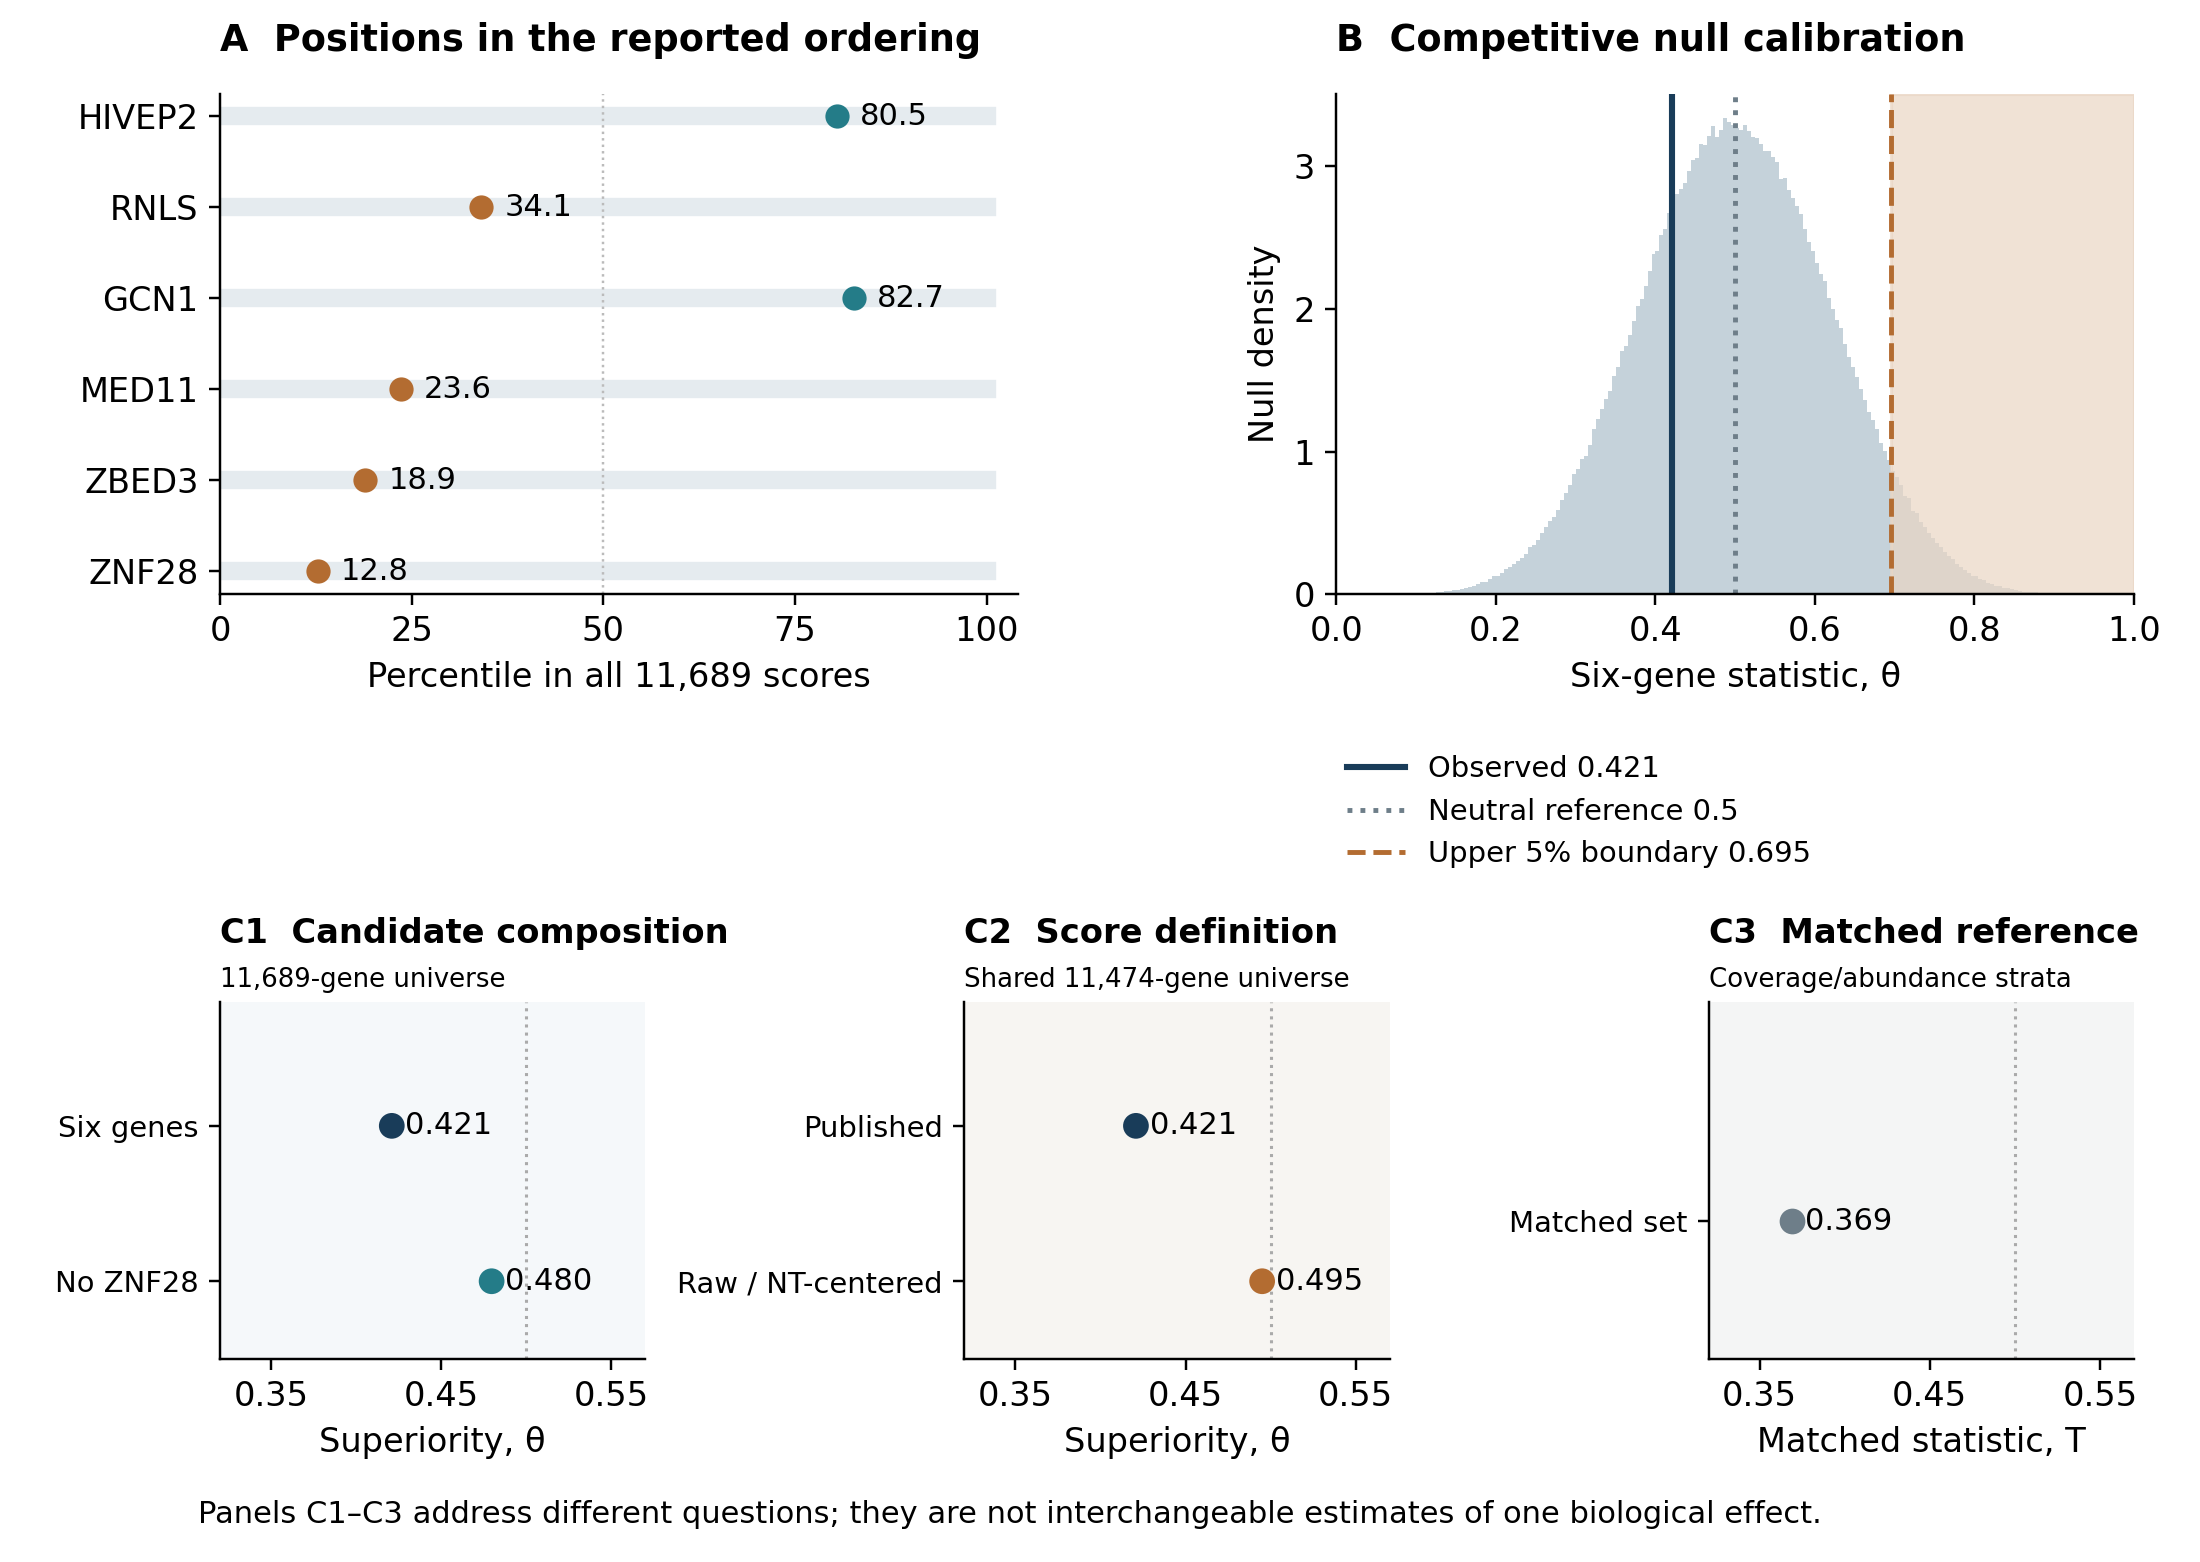
\includegraphics[width=\linewidth]{figures/transfer.png}
\par\small Figure 2. A: candidate percentile positions in the complete published ordering; colors indicate positive/negative scores, not significant discoveries. B: six-gene competitive null with observed statistic, neutral reference and upper 5\% boundary. C: separate groups distinguish candidate-composition changes from common-universe score comparisons and the conditional matched reference. Points are conditional statistics, not biological uncertainty intervals or interchangeable effect estimates.
\end{figure}
\subsection*{Functional evidence coverage}
The evidence table contains thirty-four extracted comparison records, five target-coverage records and one completed full-text source assessment [14]. Coverage and source-only records are not experiments. Seven baseline secretion comparison records concern RNLS or HIVEP2, representing two of six scored counterparts and two of eleven original targets. No adequate target-specific post-autoimmune or post-allogeneic basal/stimulated comparison was located in the assessed material (Figure 3). These counts describe evidence coverage, not biological failure rates. Bode's 2023 full text and complete supplement report metabolic, immune and graft outcomes without a direct secretion assay. Repeated target entries from a pooled experiment do not increase the number of independent studies. Detailed retrieval counts, source access and experiment-level decisions are supplementary.\par
\begin{figure}[!htbp]\centering
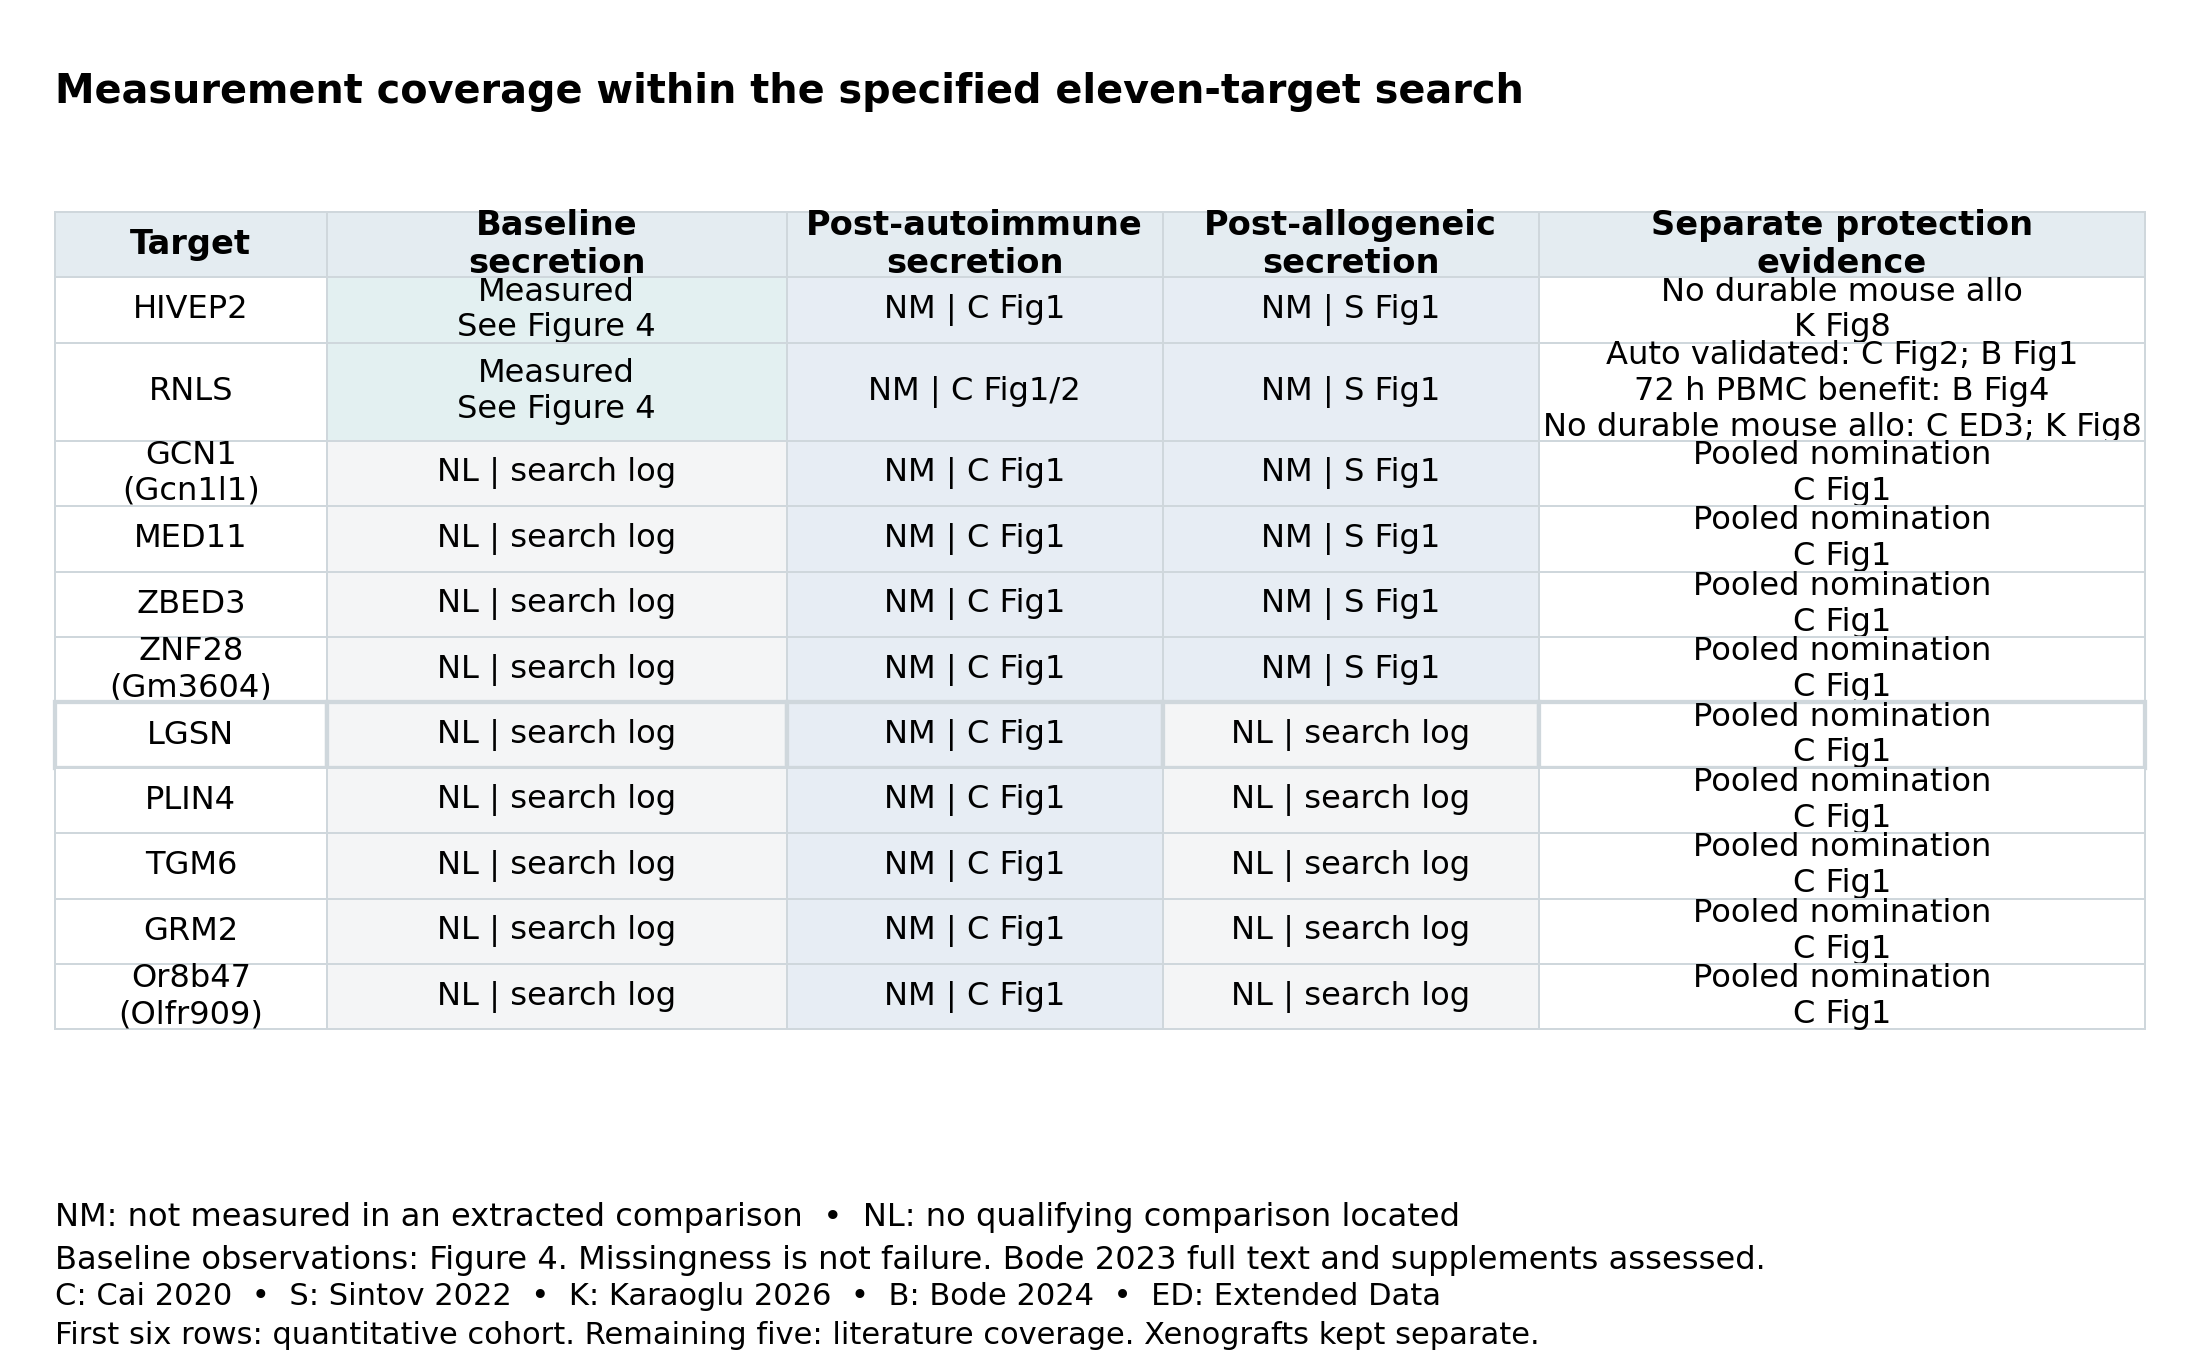
\includegraphics[width=\linewidth]{figures/evidence_matrix.png}
\par\small Figure 3. Eleven-target coverage within the specified search. Baseline measurements point to model-specific observations in Figure 4. NM: not measured for the edit in an extracted comparison; NL: no qualifying comparison located. Favorable short human PBMC co-culture survival and absent durable mouse allogeneic protection are distinct outcomes. First six rows form the quantitative cohort; remaining five are literature targets.
\end{figure}
\begin{figure}[!htbp]\centering
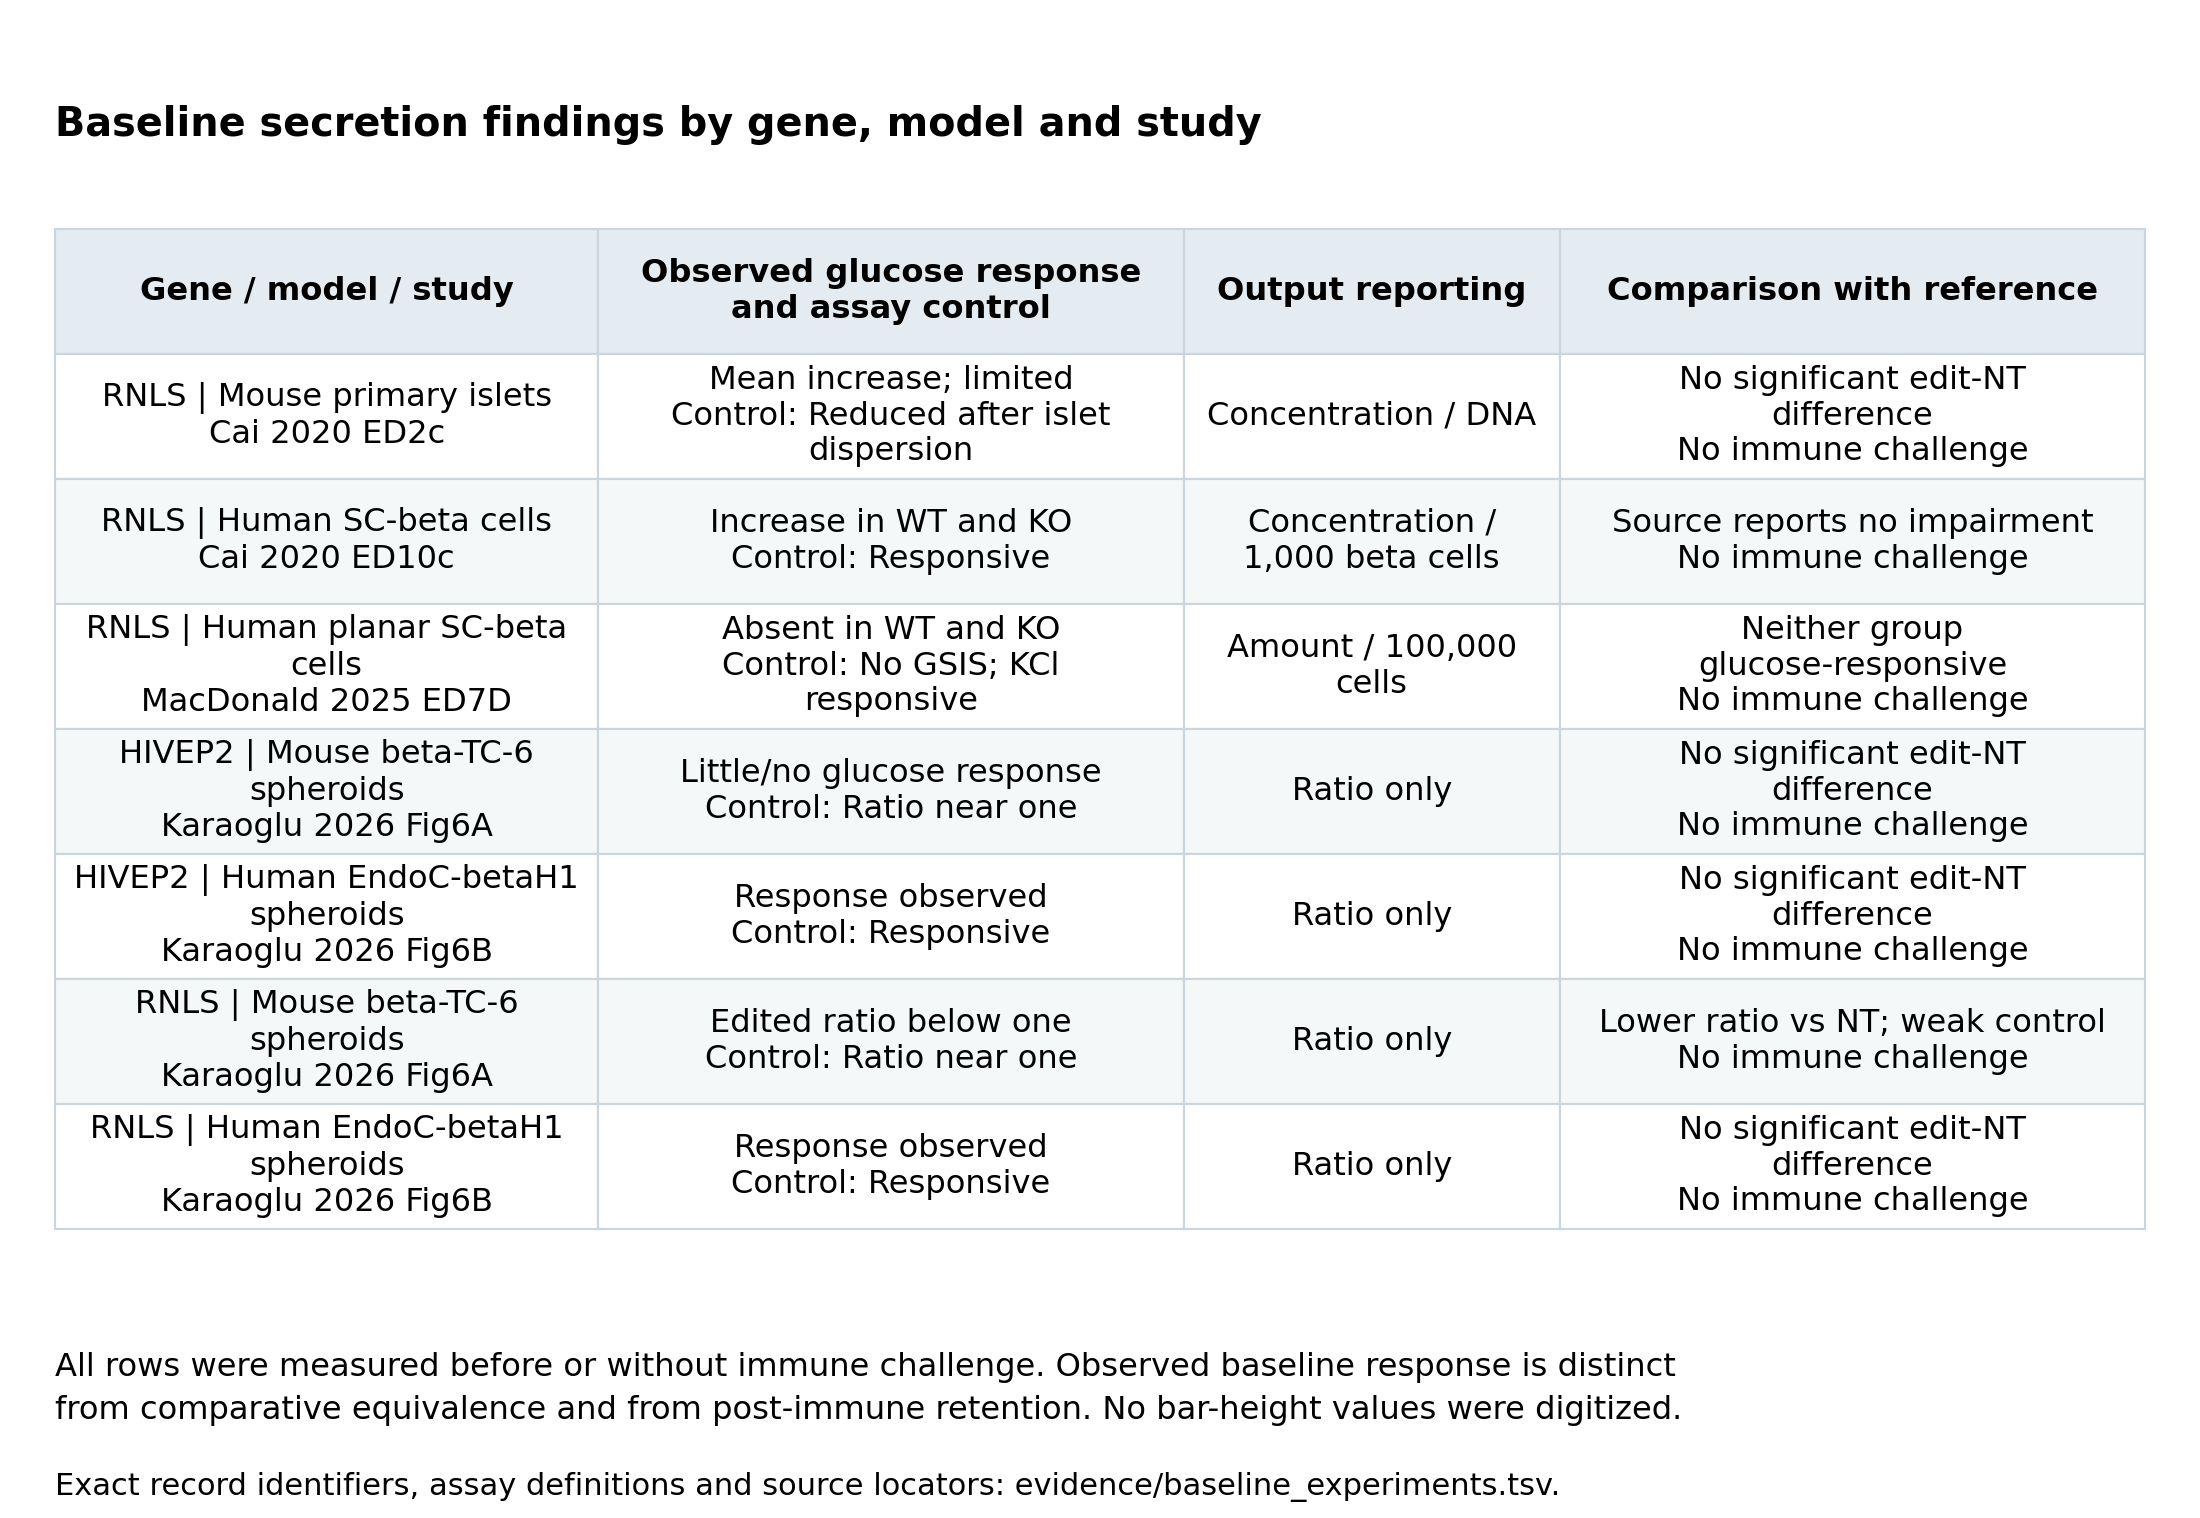
\includegraphics[width=\linewidth]{figures/baseline_experiments.png}
\par\small Figure 4. Baseline findings by gene, model and study. Observed glucose responsiveness, control performance, comparative result and output reporting remain distinct. A favorable baseline observation can be informative without establishing equivalence or post-immune retention. All displayed comparisons precede or omit immune challenge. Values were not inferred from bar heights; exact source locators accompany each row.
\end{figure}
Cai's human SC-beta cells showed glucose-responsive secretion in both wild-type and RNLS-knockout preparations, with the source reporting no impairment (Extended Data Figure 10c) [1]. This is favorable baseline evidence; absence of a formal noninferiority analysis does not erase the observed response. Cai's primary mouse-islet measurements were less informative because islet dispersion reduced responsiveness. MacDonald's planar SC-beta cultures showed no glucose response in either genotype despite a KCl response, making that comparison different from Cai's responsive preparations [4]. Karaoglu's human EndoC-betaH1 spheroids responded to glucose, with no significant edited-control difference for RNLS or HIVEP2; the mouse beta-TC-6 controls were weakly responsive, and RNLS-edited mouse spheroids had a lower ratio [3]. Figure 4 preserves these gene--model--study distinctions and separates normalized absolute output from ratios alone. All seven comparisons preceded or omitted immune challenge, so their baseline observations do not demonstrate retained function after attack.\par
RNLS protection is context dependent. Cai's mouse experiments supported autoimmune protection but not allogeneic graft protection [1]; RNLS/HIVEP2 mouse spheroids likewise lacked durable allogeneic protection [3]. Bode's human SC-derived beta-like cultures showed higher live CD45-negative cell counts and live/dead ratios after 72 hours of IL2-stimulated, HLA-mismatched PBMC exposure [13]. This favorable short co-culture result is neither a beta-cell-marker-gated endpoint nor durable graft protection, and it does not measure secretion. Human-to-mouse grafts in the spheroid study are xenogeneic [3]. Outside the cohort, CXCL10 supports allogeneic protection, but its post-PBMC post-glucose output lacks a contemporaneous basal/stimulated comparison [2]. A pooled STAT1 signal failed in separate clonal protection follow-up. Screen persistence, independent protection and retained function remain distinct observations.\par
\FloatBarrier
\section*{Discussion}
Autoimmune-screen nomination alone should not be treated as evidence of established allogeneic protection. The nominated-set test detected no enrichment, while no qualifying post-immune functional-retention comparison was located in the assessed material. Nondetection does not rule out useful candidates or preclude experimental prioritization based on biological plausibility, feasibility or expected information. This focused reanalysis contributes a defined comparison, transparent coverage accounting and an experiment-specific evidence map.\par
The candidates pose different next questions. GCN1's positive score and high matched position motivate independent engineering and validation. HIVEP2 raises a discrepancy between its screen direction and model-specific follow-up. RNLS provides a benchmark for known context dependence. These are investigative roles, not demonstrated successes.\par
A discriminating extension would test separately verified edits in one glucose-responsive human beta-cell product under unchallenged, autoimmune and allogeneic conditions. Independent edited preparations, differentiation batches and immune donors should supply biological replication; technical wells do not. Measure survival, total basal/stimulated output, viable beta-cell mass and secretion per surviving cell, before and after challenge where feasible. Responsive survivors with little total graft output differ from a useful retained graft. A prespecified functional reference and justified retention margin, assessed through direct edit-by-challenge comparisons, would distinguish context-specific protection from persistence with impaired function.\par
The six-gene cohort is small and selected; the five unscored or unmapped targets cannot be treated as failures. Multiple biological and screening differences preclude attribution specifically to rejection type. Rank references do not propagate experimental uncertainty or dependence, and matched strata address only selected covariates. The count diagnostic has unresolved donor and model limitations. The bounded search may miss relevant experiments; located studies sometimes lack absolute-output uncertainty or contain inconsistent captions. Broader biological claims require harmonized observations rather than further simulations.\par
\section*{Reproducibility and scope}
The package supplies mapping outcomes, score tables, frozen primary and secondary protocols, search logs, source commitments, code and pinned dependencies. The primary plan was locally frozen before candidate-score inspection; secondary analyses were specified after that result was known. Neither was externally preregistered. README.md documents offline reconstruction from the retained source cache; supporting documents retain implementation and assay detail.\par
AI assisted retrieval, coding, extraction, writing and internal checking. No external specialist validation, new experiment or clinical endpoint is claimed. The byline identifies the responsible organization.\par
\section*{References}
{\small [1] Cai et al. (2020). Genome-scale in vivo CRISPR screen identifies RNLS as a target for beta cell protection in type 1 diabetes. Nature Metabolism. DOI: 10.1038/s42255-020-0254-1.\par}
{\small [2] Sintov et al. (2022). Whole-genome CRISPR screening identifies genetic manipulations to reduce immune rejection of stem cell-derived islets. Stem Cell Reports. DOI: 10.1016/j.stemcr.2022.08.002.\par}
{\small [3] Karaoglu et al. (2026). Single-gene knockout of RNLS or HIVEP2 are insufficient to protect beta-cell spheroids from allo- and xeno-rejection. Frontiers in Immunology. DOI: 10.3389/fimmu.2026.1759835.\par}
{\small [4] MacDonald et al. (2025). Renalase inhibition defends against acute and chronic beta cell stress by regulating cell metabolism. Molecular Metabolism 95:102115. DOI: 10.1016/j.molmet.2025.102115.\par}
{\small [5] Mouse Genome Informatics / Alliance of Genome Resources. HOM\_MouseHumanSequence.rpt; Gcn1 MGI:2444248; Gm3604 MGI:3781781. Frozen mapping snapshot retrieved 25 October 2026 UTC (24 October America/New\_York); current aliases documented separately.\par}
{\small [6] NCBI GEO. GSE200085 / GSM6008413. Guide counts, sample information and CP0043 construct reference; Broad GPP CP0043 annotations and Addgene Mouse GeCKOv2 A. Exact versions and hashes in sources.tsv.\par}
{\small [7] Mann HB, Whitney DR (1947). On a test of whether one of two random variables is stochastically larger than the other. Annals of Mathematical Statistics 18:50--60. DOI: 10.1214/aoms/1177730491.\par}
{\small [8] Greenland S et al. (2016). Statistical tests, P values, confidence intervals, and power: a guide to misinterpretations. European Journal of Epidemiology 31:337--350. DOI: 10.1007/s10654-016-0149-3.\par}
{\small [9] Wu D, Smyth GK (2012). Camera: a competitive gene set test accounting for inter-gene correlation. Nucleic Acids Research 40:e133. DOI: 10.1093/nar/gks461.\par}
{\small [10] Lakens D (2017). Equivalence tests: a practical primer for t tests, correlations, and meta-analyses. Social Psychological and Personality Science 8:355--362. DOI: 10.1177/1948550617697177.\par}
{\small [11] Page MJ et al. (2021). The PRISMA 2020 statement: an updated guideline for reporting systematic reviews. BMJ 372:n71. DOI: 10.1136/bmj.n71.\par}
{\small [12] Rethlefsen ML et al. (2021). PRISMA-S: an extension to the PRISMA Statement for Reporting Literature Searches in Systematic Reviews. Systematic Reviews 10:39. DOI: 10.1186/s13643-020-01542-z.\par}
{\small [13] Bode K, Wei S, Gruber I, Li J, Kissler S, Yi P (2024). Beta cells deficient for Renalase counteract autoimmunity by shaping natural killer cell activity. Frontiers in Immunology 15:1403752. DOI: 10.3389/fimmu.2024.1403752.\par}
{\small [14] Bode K et al. (2023). Protective Renalase Deficiency in beta-Cells Shapes Immune Metabolism and Function in Autoimmune Diabetes. Diabetes 72:1127--1143. DOI: 10.2337/db23-0030.\par}
\end{document}
